\documentclass{article}


% if you need to pass options to natbib, use, e.g.:
%     \PassOptionsToPackage{numbers, compress}{natbib}
% before loading neurips_2023


% ready for submission
\usepackage{neurips_2024}


% to compile a preprint version, e.g., for submission to arXiv, add add the
% [preprint] option:
%     \usepackage[preprint]{neurips_2023}


% to compile a camera-ready version, add the [final] option, e.g.:
%     \usepackage[final]{neurips_2023}


% to avoid loading the natbib package, add option nonatbib:
%    \usepackage[nonatbib]{neurips_2023}


\usepackage[utf8]{inputenc} % allow utf-8 input
\usepackage[T1]{fontenc}    % use 8-bit T1 fonts
\usepackage{hyperref}       % hyperlinks
\usepackage{url}            % simple URL typesetting
\usepackage{booktabs}       % professional-quality tables
\usepackage{amsfonts}       % blackboard math symbols
\usepackage{nicefrac}       % compact symbols for 1/2, etc.
\usepackage{microtype}      % microtypography
\usepackage{xcolor}         % colors
\usepackage{graphicx}

\title{Diffusion Probabilistic Models for Super Resolution Microscopy}


% The \author macro works with any number of authors. There are two commands
% used to separate the names and addresses of multiple authors: \And and \AND.
%
% Using \And between authors leaves it to LaTeX to determine where to break the
% lines. Using \AND forces a line break at that point. So, if LaTeX puts 3 of 4
% authors names on the first line, and the last on the second line, try using
% \AND instead of \And before the third author name.


\author{%
  David S.~Hippocampus\thanks{Use footnote for providing further information
    about author (webpage, alternative address)---\emph{not} for acknowledging
    funding agencies.} \\
  Department of Computer Science\\
  Cranberry-Lemon University\\
  Pittsburgh, PA 15213 \\
  \texttt{hippo@cs.cranberry-lemon.edu} \\
  % examples of more authors
  % \And
  % Coauthor \\
  % Affiliation \\
  % Address \\
  % \texttt{email} \\
  % \AND
  % Coauthor \\
  % Affiliation \\
  % Address \\
  % \texttt{email} \\
  % \And
  % Coauthor \\
  % Affiliation \\
  % Address \\
  % \texttt{email} \\
  % \And
  % Coauthor \\
  % Affiliation \\
  % Address \\
  % \texttt{email} \\
}


\begin{document}


\maketitle


\begin{abstract}
Single-molecule localization microscopy (SMLM) techniques are a mainstay of fluorescence microscopy and can be used to produce a pointillist representation of living cells at diffraction-unlimited precision. Classical SMLM approaches leverage the deactivation of fluorescent tags, followed by spontaneous or photoinduced reactivation, which can be used to estimate of the density of a tagged biomolecule in cellular compartments. Standard SMLM localization algorithms based on maximum likelihood estimators or least squares optimization require tight control of activation and reactivation to maintain sparse emitters, presenting a tradeoff between imaging speed and labeling density. Deep models have generalized SMLM to densely labeled structures, yet uncertainty quantification is still lacking. Recently, denoising diffusion probabilstic models (DDPMs) have been adapted conditional super resolution tasks, demonstrating promising results in detail reconstruction, while directly providing uncertainties in model predictions. Here, we adapt DDPM to the task of single molecule localization, and demonstrate that DDPM approaches the Cramer-Rao lower bound on localization uncertainty over a wide range of experimental conditions.
\end{abstract}

\section{Introduction}
Single molecule localization microscopy (SMLM) relies on the temporal resolution of fluorophores whose spatially overlapping point spread functions would otherwise render them unresolvable at the detector. Common strategies for the temporal separation of molecules involve transient intramolecular rearrangements to switch from dark to fluorescent states or the exploitation of non-emitting molecular radicals. Estimation of molecular coordinates in SMLM is acheived by modeling the optical impulse response of the imaging system. However, dense localization suffers from the curse of dimensionality - the parameter space volume grows exponentially with the number of molecules, which is often unknown a priori. Exploration of this high dimensional parameter space in dense SMLM is often intractable. 

Previous approaches to this issue has been to predict super-resolution images from a sparse set of localizations with conditional generative adversarial networks (Ouyang 2018) or direct prediction of coordinates using deep neural networks (Nehme 2020; Speiser 2021). However, diffusion models are an appealing alternative because they infer a distribution of deconvolved images that are compatible with an observation. Although conditional VAEs and conditional GANs can provide a distribution of deconvolved images, both are known to suffer from mode collapse and produce insufficient diversity in their outputs. Diffusion models are a recently developed alternative to VAEs and GANs that excel at producing diverse samples and have been successfully applied to solve inverse problems. Here, we present a novel diffusion model for deconvolution in single molecule localization microscopy. The first stage of our algorithm performs interpolation by computing second order coherence of pixel pairs. Subsequent stages cast localization as a conditional image refinement task, realized by a U-Net model trained on denoising at various noise levels. 

This is followed by coordinate refinement by a gradient-based Markov Chain Monte Carlo (MCMC) scheme, known as Langevin dynamics.


\section{Denoising Diffusion Probabilistic Model for SMLM}

\begin{figure}
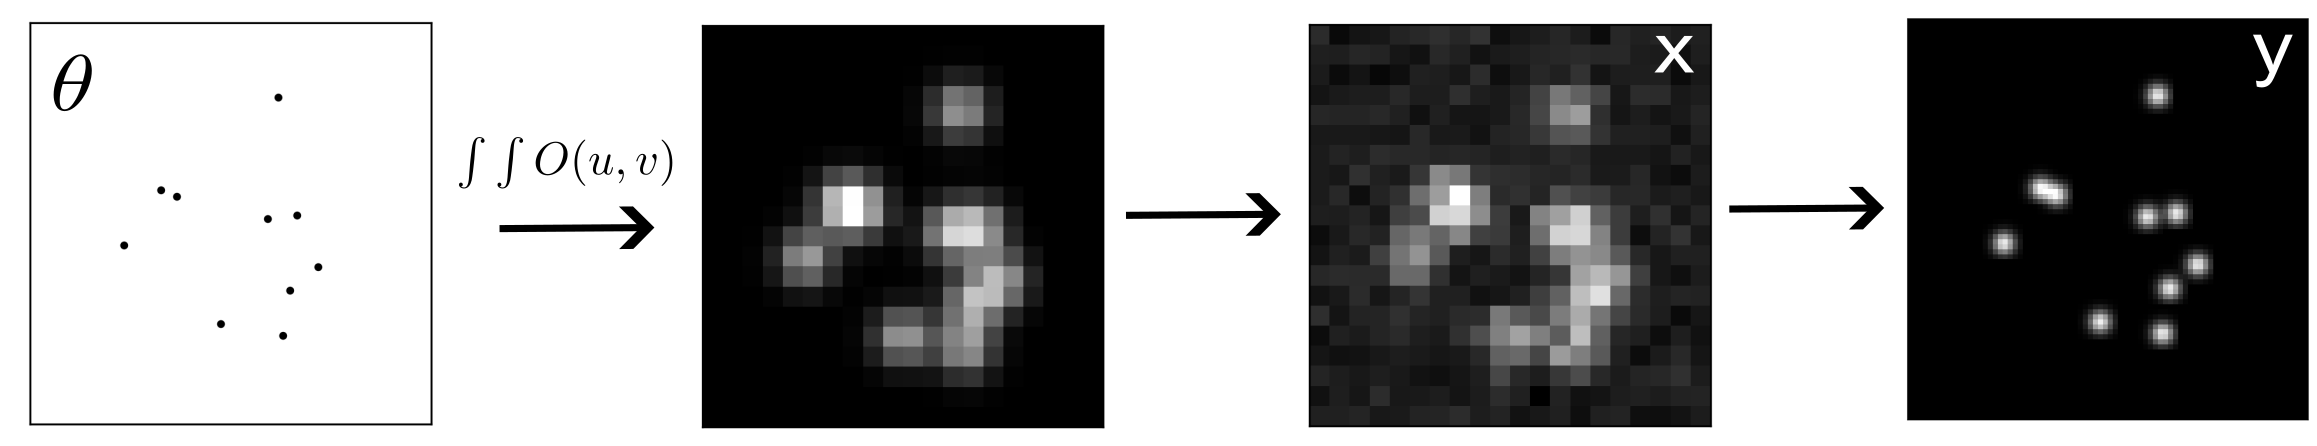
\includegraphics[scale=0.5]{Generation.png}
\end{figure}

We consider datasets $(\theta_{i}, \bold{x}_i,\bold{y}_i)_{i=1}^{N}$ of observed images $\bold{x}_i$ and kernel density estimate (KDE) images $\bold{y}_{i}$, given an underlying set of object coordinates $\theta_{i}$. Observations $\bold{x}_i$ are generated from $\theta_{i}=(r_{1},...,r_{N})$ under an image degradation model $F$. We aim to develop a framework for sampling from $p(\bold{y}_{i}|\bold{x}_{i})$ and inference of $\theta_{i}$, while fulfilling a resolution criterion under the condition $|r_{i}-r_{j}| \geq \epsilon ; \forall (i,j)$. 

\subsection{Degradation Model}

The central objective of single molecule localization microscopy is to infer a set of molecular coordinates $\theta$ from noisy, low resolution images $\bold{x}$. We define an abstract image stochastic degradation function $F$ such that $\bold{x} = F(\theta)$. In the following paragraphs, we define such a function $F$. 

In fluorescence microscopy, each pixel follows Poisson statistics, with expected value

\begin{equation}
\omega = i_{0}\int O(u)du\int O(v)dv
\end{equation}

where $i_{0} = \eta N_{0}\Delta$. The optical impulse response $O(u,v)$ is often approximated as a 2D isotropic Gaussian with standard deviation $\sigma$ (Zhang 2007). The parameter $\eta$ is the photon detection probability of the sensor and $\Delta$ is the exposure time. $N_{0}$ represents the number of photons emitted.

For a fluorescent emitter located at $\theta = (u_{0},v_{0})$, we have that

\begin{equation}
\int O(u)du = \frac{1}{2}\left(\mathrm{erf}\left(\frac{u_{k}+\frac{1}{2}-u_{0}}{\sqrt{2}\sigma}\right) -\mathrm{erf}\left(\frac{u_{k}-\frac{1}{2}-u_{0}}{\sqrt{2}\sigma}\right)\right)
\end{equation}

where we have used the common definition $\mathrm{erf}(z) = \frac{2}{\sqrt{\pi}}\int_{0}^{t}e^{-t^{2}}dt$. For the sake of generality, the number of photoelectrons at a pixel $k$, $\bold{s}_k$, is  multiplied by a gain factor $g_k \;[\mathrm{ADU}/e^{-}]$, which is often unity. The readout noise per pixel $\zeta_{k}$ can be Gaussian with some pixel-specific offset $o_{k}$ and variance $\sigma_{k}^{2}$. Ultimately, we have a Poisson component of the signal, which scales with $N_{0}$ and may have Gaussian component, which does not. Therefore, in a single exposure, we measure: 

\begin{equation}
\bold{x}_t = \bold{s}_t + \bold{\zeta}
\end{equation}

What we are after is the likelihood $p(\bold{x}_{t}|\theta)$ where $\theta$ are the molecular coordinates. Fundamental probability theory states that the distribution of $\bold{x}_{k}$ is the convolution of the distributions of $\bold{s}_{k}$ and $\zeta_{k}$,

\begin{equation}
p(\bold{x}_{t}|\theta) = A\sum_{q=0}^{\infty} \frac{1}{q!}e^{-\omega_{k}}\omega_{k}^{q}\frac{1}{\sqrt{2\pi}\sigma_{k}}e^{-\frac{(\bold{x}_{k}-g_{k}q-o_{k})}{2\sigma_{k}^{2}}}
\end{equation}

where $P(\zeta_{k}) = \mathcal{N}(o_{k},\sigma_{k}^{2})$ and $P(S_{k}) = \mathrm{Poisson}(g_{k}\omega_{k})$,  $A$ is some normalization constant. In practice, (4) is difficult to work with, so we look for an approximation. We will use a Poisson-Normal approximation for simplification. Consider,

\begin{equation}
\zeta_{k} - o_{k} + \sigma_{k}^{2} \sim \mathcal{N}(\sigma_{k}^{2},\sigma_{k}^{2}) \approx \mathrm{Poisson}(\sigma_{k}^{2})
\end{equation}

Since $\bold{x}_{k} = \bold{s}_{k} + \zeta_{k}$, we transform $\bold{x}_{k}' = \bold{x}_{k} - o_{k} + \sigma_{k}^{2}$, which is distributed according to 

\begin{equation}
\bold{x}_{k}' \sim \mathrm{Poisson}(\omega_{k}')
\end{equation}

where $\omega_{k}' = g_{k}\omega_{k} + \sigma_{k}^{2}$. This result can be seen from the fact the the convolution of two Poisson distributions is also Poisson. The quality of this approximation will degrade with decreasing signal level, since the Poisson distribution does not retain its Gaussian shape at low expected counts. Nevertheless, the quality of the approximation can be predicted by the Komogonov distance between the convolution distribution (4).

\subsection{The Information Bottleneck for Localization}

\begin{figure}
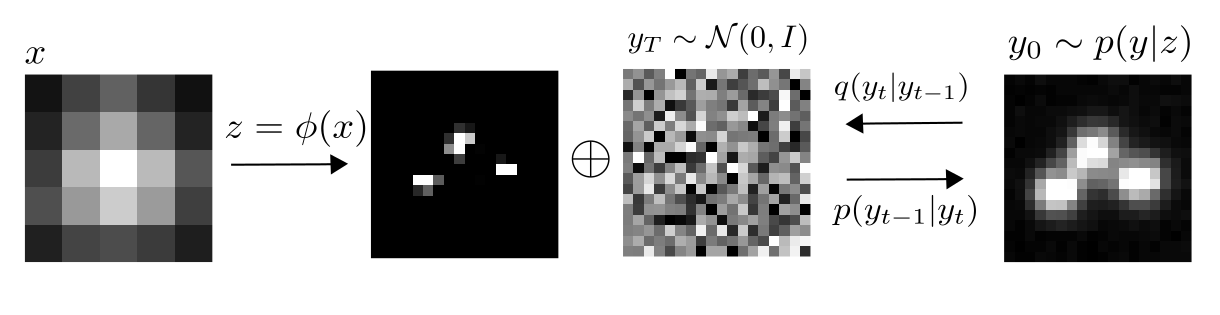
\includegraphics[scale=4.0]{Denoise.png}
\end{figure}

Inversion of the degradation function $F$ is generally intractable, particularly when fluorescent molecules are dense within the field of view. This difficulty arises because the parameter $\bold{\theta}$ is typically of large and unknown dimension, rendering maximum likelihood estimation or Markov Chain Monte Carlo sampling computationally difficult. Previous solutions to this problem leverage convolutional neural networks (CNNs) to infer coordinates directly by learning a deterministic image transformation $F^{-1}$, which we refer to as a "localization map" (Nehme 2021). Such methods faithfully capture the information content in degraded images; however, such methods apply arbitrary thresholding to the CNN localization map, potentially creating erroneous localizations, and do not permit sampling. 

We seek a generative approach, which casts localization as an image restoration problem, where a high resolution kernel density estimate $\bold{y}$ is reconstructed from a low resolution image $\bold{x}$. Building on previous efforts, we utilize a CNN learns a representation which compresses $\bold{x}$ while preserving the relevant information to the prediction of $\bold{y}$. We use the Fisher information as the information theoretic criteria (Chao 2016). The generative model (6) is also convenient for computing the Fisher information matrix (Smith 2010) and thus the Cramer-Rao lower bound, which bounds the variance of a statistical estimator of $\theta$, from below. The Fisher information is

\begin{equation}
\mathcal{I}_{ij}(\theta) = \mathbb{E}\left(\frac{\partial \ell}{\partial\theta_{i}}\frac{\partial\ell}{\partial\theta_{j}}\right) = \sum_{k}\frac{1}{\omega_{k}'}\frac{\partial \omega_{k}'}{\partial\theta_{i}}\frac{\partial \omega_{k}'}{\partial\theta_{j}}
\end{equation}

where the log-likelihood is $\ell (\bold{x}_{t}|\theta)$.

\subsection{Denoising Diffusion Probabilistic Model}

Denoising diffusion probabilistic models (DDPM) have emerged as powerful generative models, exceeding GANs and VAEs in a variety of generative modeling tasks. Nevertheless, learning diffusion models directly in data space can limit expressivity of the model (Vahdat 2021). Therefore, we build on previous approaches by using a CNN to compute a latent representation $\bold{z}_{i}$. A denoising diffusion probabilistic model (DDPM) is then used to model the distribution $P_{\Phi}(\bold{y}|\bold{z})$. 

Let $\bold{y}_{0} = \sum_{i=1}^{n} \bold{\omega}_{n}(\sigma)$ be a density estimate of the molecular distribution. The \emph{forward} process is the joint distribution $p_{\theta}(\bold{y}_{0:T})$, which is Markovian. 

\begin{equation}
q(\bold{y}_{t}|\bold{y}_{0}) = \prod_{t=1}^{T}q(\bold{y}_{t}|\bold{y}_{t-1}) \;\;\; q(\bold{y}_{t}|\bold{y}_{t-1}) = \mathcal{N}\left(\bold{y}_{t-1},\sqrt{\alpha_{t}}\bold{y}_{t-1},(1-\alpha_{t})I\right)
\end{equation}

We optimize a denoising model $f_{\theta}$ which takes as input an interpolated low-resolution input $\bold{y}$ and a noisy input $\bold{y}_{T}$. 

\begin{equation}
p_{\theta}(\bold{y}_{0:T}) = p_{\theta}(\bold{y}_{T})\prod_{t=1}^{T} p_{\theta}(\bold{y}_{t-1}|\bold{y}_{t}) \;\;\; p_{\theta}(\bold{y}_{t-1}|\bold{y}_{t}) = \mathcal{N}\left(\bold{y}_{t-1},\mu_{\theta}(\bold{y}_{t},\gamma_{t}),\sigma^{2}_{t}I\right)
\end{equation}

where $\gamma_{t}=\prod_{i=1}^{t}\alpha_{t}$. Note that the model $\theta$ is not a function of $t$. The mean of the transition density reads

\begin{equation}
\mu_{\theta}(\bold{x}_{t},\bold{y},\gamma_{t}) = \frac{1}{\sqrt{\alpha_{t}}}\left(\bold{y}_t-\frac{1-\alpha_{t}}{\sqrt{1-\gamma_{t}}}f_{\theta}(\bold{x}_{t},\gamma_{t})\right)
\end{equation}


\section{Experiments}


\begin{figure}
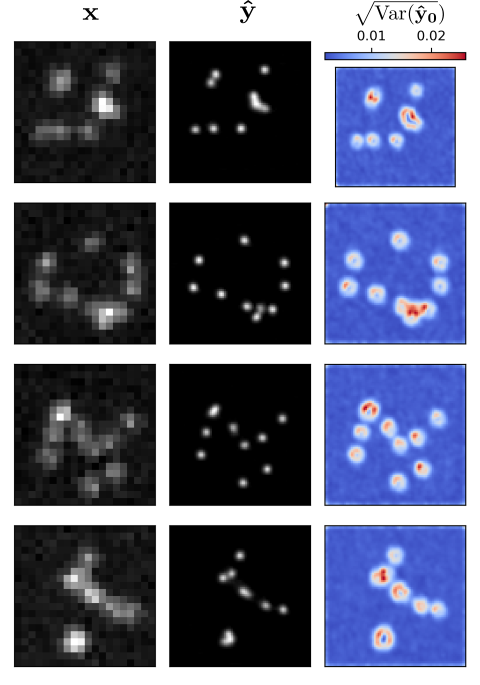
\includegraphics[scale=0.6]{Samples.png}
\end{figure}



\end{document}